\documentclass[11pt,a4paper]{article}

% --- Geometry & Layout ---
\usepackage[margin=1in]{geometry}
\usepackage{parskip}
\usepackage[T1]{fontenc}
\usepackage[utf8]{inputenc}

% --- Section Formatting ---
\usepackage{titlesec}
\usepackage{tocloft}

% --- Colors & Boxes ---
\usepackage[dvipsnames,svgnames]{xcolor}
\usepackage[most]{tcolorbox}

% --- Lists & Tables ---
\usepackage{enumitem}
\usepackage{booktabs}
\usepackage{longtable}
\usepackage{tabularx}
\usepackage{array}

% --- Code Listings ---
\usepackage{listings}

% --- Graphics ---
\usepackage{tikz}
\usetikzlibrary{arrows.meta,positioning,shapes.geometric,fit,calc,backgrounds}

% --- Hyperlinks ---
\usepackage[colorlinks=true,linkcolor=NavyBlue,urlcolor=RoyalBlue,citecolor=NavyBlue]{hyperref}

% --- Headers & Footers ---
\usepackage{fancyhdr}
\pagestyle{fancy}
\fancyhf{}
\fancyhead[L]{\small\textsc{Levshell Design Language}}
\fancyhead[R]{\small\textsc{v0.2 --- In Progress}}
\fancyfoot[C]{\thepage}
\renewcommand{\headrulewidth}{0.4pt}

% ===========================================================================
% Color Definitions — these mirror the proposed shell palette
% ===========================================================================

% Warm Dark default palette (finalized)
\definecolor{bg}{HTML}{1A1B26}
\definecolor{bgdark}{HTML}{16161E}
\definecolor{surface}{HTML}{24283B}
\definecolor{surfaceraised}{HTML}{2F3549}
\definecolor{overlay}{HTML}{3B4261}
\definecolor{fg}{HTML}{C0CAF5}
\definecolor{fgmuted}{HTML}{565F89}
\definecolor{fgsubtle}{HTML}{737AA2}

\definecolor{primary}{HTML}{7AA2F7}
\definecolor{primaryvar}{HTML}{5A7FD4}
\definecolor{secondary}{HTML}{BB9AF7}
\definecolor{secondaryvar}{HTML}{9D7CD8}
\definecolor{tertiary}{HTML}{7DCFFF}

\definecolor{success}{HTML}{9ECE6A}
\definecolor{warning}{HTML}{E0AF68}
\definecolor{error}{HTML}{F7768E}
\definecolor{info}{HTML}{2AC3DE}

\definecolor{onprimary}{HTML}{1A1B26}
\definecolor{onsurface}{HTML}{C0CAF5}
\definecolor{outline}{HTML}{3B4261}

% Spec document styling
\definecolor{levblue}{HTML}{7AA2F7}
\definecolor{levpurple}{HTML}{BB9AF7}
\definecolor{levgreen}{HTML}{9ECE6A}
\definecolor{levorange}{HTML}{E0AF68}
\definecolor{levred}{HTML}{F7768E}
\definecolor{codebg}{HTML}{F0F0F4}

% ===========================================================================
% Custom Environments
% ===========================================================================
\newtcolorbox{designbox}[1][]{
  colback=levblue!5, colframe=levblue!60!black,
  fonttitle=\bfseries, title={#1}, arc=2pt, boxrule=0.5pt,
  left=6pt, right=6pt, top=4pt, bottom=4pt,
}

\newtcolorbox{principlebox}[1][]{
  colback=levpurple!5, colframe=levpurple!60!black,
  fonttitle=\bfseries, title={#1}, arc=2pt, boxrule=0.5pt,
  left=6pt, right=6pt, top=4pt, bottom=4pt,
}

\newtcolorbox{notebox}[1][]{
  colback=levorange!5, colframe=levorange!60!black,
  fonttitle=\bfseries, title={#1}, arc=2pt, boxrule=0.5pt,
  left=6pt, right=6pt, top=4pt, bottom=4pt,
}

\newtcolorbox{swatch}[2][]{
  colback=#2, colframe=#2!80!black,
  fonttitle=\bfseries\color{white}, title={#1}, arc=2pt, boxrule=0.5pt,
  left=4pt, right=4pt, top=2pt, bottom=2pt,
  width=3.2cm, height=1.4cm,
}

% --- Code Listing Style ---
\lstset{
  backgroundcolor=\color{codebg}, basicstyle=\ttfamily\small,
  breaklines=true, frame=single, rulecolor=\color{gray!40},
  keywordstyle=\color{NavyBlue}\bfseries,
  commentstyle=\color{OliveGreen}\itshape,
  stringstyle=\color{BrickRed},
  showstringspaces=false, tabsize=2,
  xleftmargin=4pt, xrightmargin=4pt, aboveskip=8pt, belowskip=8pt,
}

% --- Title Formatting ---
\titleformat{\section}{\Large\bfseries\color{NavyBlue}}{\thesection}{1em}{}[\vspace{-4pt}\textcolor{levblue}{\rule{\textwidth}{0.5pt}}]
\titleformat{\subsection}{\large\bfseries\color{NavyBlue!80}}{\thesubsection}{1em}{}
\titleformat{\subsubsection}{\normalsize\bfseries\color{NavyBlue!60}}{\thesubsubsection}{1em}{}

\renewcommand{\cftsecleader}{\cftdotfill{\cftdotsep}}

% ===========================================================================
\begin{document}

% --- Title Page ---
\begin{titlepage}
\centering
\vspace*{2cm}

{\Huge\bfseries\color{NavyBlue} Levshell\par}
\vspace{0.5cm}
{\Large\color{NavyBlue!70} Design Language Specification\par}

\vspace{1cm}
\textcolor{levblue}{\rule{0.6\textwidth}{1pt}}

\vspace{1.5cm}
{\large\textsc{Companion to the Engineering Specification}\par}
\vspace{0.3cm}
{\normalsize Version 0.2 --- In Progress\par}
\vspace{0.3cm}
{\normalsize\today\par}

\vspace{3cm}

\begin{principlebox}[Design Philosophy]
A shell for the 20-hour study day. Every pixel earns its place. Beauty is not decoration---it is the reduction of cognitive friction to zero. The shell should feel like a calm, intelligent surface: warm in the dark, quiet when you're focused, and unmistakably present when you need it.
\end{principlebox}

\vspace{2cm}

{\small\textit{This document defines the visual language, component anatomy, motion system,\\and design tokens that govern every rendered surface in Levshell.\\Design decisions are being iteratively finalized\\in preparation for Phase~1 QML implementation.}\par}

\vfill
\end{titlepage}

% --- Table of Contents ---
\newpage
\tableofcontents
\newpage


% ===========================================================================
\section{Scope and Purpose}
\label{sec:scope}

This document is the visual companion to the Levshell engineering specification. It defines every design decision that affects what the user sees: colors, typography, spacing, motion, component anatomy, iconography, and the visual grammar for context-aware state changes.

\subsection{What This Document Covers}

\begin{enumerate}[leftmargin=1.5em, itemsep=3pt]
  \item \textbf{Color system.} Semantic color roles, palette definition, dark/light mode strategy, accent-per-workspace mapping, blur/transparency interaction.
  \item \textbf{Typography.} Font families, type scale, weights, tabular figures, per-context typographic treatment.
  \item \textbf{Spacing and density.} Base unit grid, widget internal metrics, density mode definitions (full/compact/hidden), responsive behavior.
  \item \textbf{Motion and animation.} Easing curves, duration scale, what animates vs.\ what snaps, motion principles.
  \item \textbf{Widget anatomy.} Component library defining every widget in every prominence state (icon-only, compact, visible, expanded) and every health state (normal, stale, error, unavailable).
  \item \textbf{Iconography.} Icon style, size scale, color behavior, icon set selection.
  \item \textbf{Urgency and escalation grammar.} The visual vocabulary for ``quiet until important'': how widgets escalate from ambient to attention-demanding.
  \item \textbf{Focus and ambient mode.} How the shell's visual tone shifts during focus sessions, compact mode, and presentation mode.
  \item \textbf{Theming architecture.} How all of the above is parameterized into theme files that users can override, and how the global color scheme propagates to GTK, Qt, terminals, and Sway borders.
  \item \textbf{Dropdown and overlay surfaces.} Panels, flyouts, the command palette, the notification center---their shared anatomy and how they relate to the bar.
\end{enumerate}

\subsection{Relationship to the Engineering Spec}

The engineering spec defines \emph{what} is rendered and \emph{when}. This document defines \emph{how} it looks. The QML implementer needs both: the engineering spec to know which widgets exist and what data they display, and this document to know what color, size, font, and animation to apply. Every visual token referenced here must be available as a QML property or CSS variable in the shell's theme system.

\begin{notebox}[Placeholder Status]
This document is being iteratively finalized. Sections marked with specific hex values, pixel sizes, font names, and durations represent \textbf{decided defaults} for the warm dark theme unless otherwise noted. The token \emph{structure}---which tokens exist, what they mean, how they compose---is the durable contribution of this document. Specific values for alternative themes (neutral dark, light mode) will be defined in their respective theme TOML files.
\end{notebox}


% ===========================================================================
\section{Design Principles}
\label{sec:principles}

\begin{principlebox}[Core Visual Principles]
\begin{enumerate}[leftmargin=1.5em, itemsep=4pt]
  \item \textbf{Calm by default, vivid on demand.} The resting state of the shell is low-contrast, muted, and warm. Color intensity increases only to communicate state changes, urgency, or active interaction. The user should never feel visually assaulted by their own desktop.

  \item \textbf{Information density without clutter.} A dense bar is not a cluttered bar. Density comes from systematic spacing, consistent alignment, and hierarchical typography---not from cramming text into every pixel. Every element has breathing room proportional to its importance.

  \item \textbf{The 3-second rule.} Any piece of information the user might need should be visually locatable within 3 seconds of looking at the bar. This means consistent placement, predictable grouping, and clear visual hierarchy.

  \item \textbf{Motion is functional.} Animation communicates change, guides attention, and maintains spatial continuity. It never decorates, never delays, and never loops. If removing an animation would not reduce comprehension, remove it.

  \item \textbf{Respect the dark.} This is a shell for late-night work. The default palette must be dark, warm, and easy on the eyes. Light mode exists but is secondary. Blue light should be minimized in the default theme.

  \item \textbf{Systematic, not bespoke.} Every visual decision derives from tokens (color roles, spacing units, type scale steps). No widget should contain a magic number. If a new widget needs a visual property that doesn't exist in the token system, the system is incomplete---add the token, don't hardcode the value.

  \item \textbf{Graceful degradation is visible.} When something is broken or stale, the user should know instantly, but it should not scream. Degraded states are communicated through desaturation, opacity reduction, and subtle iconography---never through red borders, flashing, or modal error dialogs.
\end{enumerate}
\end{principlebox}


% ===========================================================================
\section{Color System}
\label{sec:color}

\subsection{Palette Architecture}

The color system uses semantic roles rather than raw color values. Every QML component references a role token (e.g., \texttt{Theme.surface}, \texttt{Theme.primary}), never a hex value. Theme files map role tokens to concrete colors.

The system uses a four-group organization: backgrounds (4-tier surface hierarchy), content colors, a single primary accent with secondary/tertiary variants, and semantic state colors. The architecture is simplified relative to Material Design 3---optimized for a bar-centric shell rather than a full application toolkit.

\subsubsection{Default Palette: Warm Dark}

The default theme uses a \textbf{warm dark} palette: deep blue-purple backgrounds with warm undertones, optimized for extended late-night sessions. This direction minimizes blue light emission while maintaining sufficient contrast for legibility. The warm dark palette is the primary design target; all component designs and contrast calculations are validated against it first.

The theming system (Section~\ref{sec:theming}) supports arbitrary palette directions. Levshell ships with three built-in themes: the default warm dark (Tokyo Night-inspired), a neutral dark (true gray, no hue bias), and a light mode. Community themes can implement any aesthetic---cool dark (Nord-style), warm earth (Gruvbox-style), OLED black, or entirely novel palettes---provided they supply values for all required tokens.

\subsubsection{4-Tier Surface Hierarchy}

Surfaces use a four-level elevation system: \texttt{bg} $\to$ \texttt{surface} $\to$ \texttt{surface.raised} $\to$ \texttt{overlay}. Each tier is progressively lighter, creating visual depth without relying on drop shadows alone. The four tiers accommodate the shell's layering needs: desktop background, bar and panel backgrounds, interactive elements within panels (hovered items, cards, secondary containers), and floating elements (tooltips, popovers).

\subsubsection{Adaptive Blur and Transparency}

The bar and dropdown panels use backdrop blur with semi-transparent backgrounds by default, allowing the wallpaper to subtly show through (frosted-glass effect). This is the \emph{blur-first} visual mode.

When the system is on battery or the GPU cannot sustain blur compositing, the shell falls back to an \emph{opaque} mode: surfaces use their full color values without transparency or blur. Both modes must look intentional---opaque mode is not a degraded blur mode but an equally valid visual treatment.

The transition between blur and opaque modes is governed by the \texttt{PowerStateChanged} event from the daemon (see engineering spec Section~5.3). The visual switch uses a critically damped spring at \texttt{motion.normal} ($\sim$200ms settle) to avoid a jarring snap.

Theme tokens controlling this behavior: \texttt{bar.opacity} (default 0.80), \texttt{bar.blur\_radius} (default 30px, 0 = opaque), \texttt{bar.opacity\_battery} (default 1.0), \texttt{bar.blur\_radius\_battery} (default 0).

\subsubsection{Single Primary Accent}

The shell uses a single \texttt{primary} accent color as the dominant interactive color (active workspace indicator, focused elements, primary actions). \texttt{secondary} and \texttt{tertiary} provide variety for tags, badges, and informational highlights, but \texttt{primary} carries the visual identity. Per-workspace differentiation is achieved through the breadcrumb indicator, workspace name, and context-driven widget layout---not through per-workspace accent color overrides of the bar.

\subsection{Background and Surface Colors}

\begin{longtable}{p{3.5cm} p{3cm} p{7cm}}
\toprule
\textbf{Token} & \textbf{Default (Warm Dark)} & \textbf{Usage} \\
\midrule
\texttt{bg} & \texttt{\#1A1B26} & Screen background, deepest layer. Visible behind the bar when blur is active. \\
\texttt{bg.dark} & \texttt{\#16161E} & Below-surface shadow areas, inset containers \\
\texttt{surface} & \texttt{\#24283B} & Bar background, dropdown panel backgrounds, card containers. The primary ``canvas'' tier. \\
\texttt{surface.raised} & \texttt{\#2F3549} & Hovered items, selected states, cards within panels, secondary containers. The interactive-element tier. \\
\texttt{overlay} & \texttt{\#3B4261} & Tooltips, popovers, context menus, and any surface that floats above all others. The top tier. \\
\bottomrule
\end{longtable}

The bar itself uses \texttt{surface} as its background. In blur mode, the bar uses \texttt{surface} at \texttt{bar.opacity} (default 80\%) with a backdrop blur of \texttt{bar.blur\_radius} (default 30px), allowing the wallpaper to subtly show through. In opaque mode (battery or blur disabled), the bar uses \texttt{surface} at full opacity with no blur.

\begin{notebox}[Tier Usage Guide]
When deciding which surface tier to use for a new component: \texttt{bg} is the void behind everything. \texttt{surface} is the ground plane (bar, panels). \texttt{surface.raised} is anything interactive or nested within a surface (list items on hover, cards inside a dropdown, toggle tile backgrounds). \texttt{overlay} is anything that escapes the normal stacking order (tooltips, popovers).
\end{notebox}

\subsubsection{Wallpaper Contrast Management}

When the bar uses semi-transparent \texttt{surface} with backdrop blur, the effective background color is a blend of \texttt{surface} and whatever wallpaper content is behind the bar. Bright wallpaper regions (white, yellow, light gradients) can reduce the contrast between the blended background and \texttt{fg} text, potentially dropping below legibility thresholds.

Two mechanisms ensure text remains legible regardless of wallpaper content:

\begin{enumerate}[leftmargin=1.5em, itemsep=3pt]
  \item \textbf{Inner shadow contrast floor.} The bar renders a thin, dark inner shadow along its bottom edge (1--2px, \texttt{bg.dark} at 30\% opacity). This provides a subtle but guaranteed contrast anchor at the bar's visual boundary, similar to the technique used by macOS's menu bar. The shadow is imperceptible on dark wallpapers and becomes functionally important on light ones.

  \item \textbf{Minimum effective contrast requirement.} The combination of \texttt{surface} at \texttt{bar.opacity} over a worst-case wallpaper (pure white, \texttt{\#FFFFFF}) must produce an effective background color that achieves at least \textbf{4.5:1} contrast ratio with \texttt{fg} text (WCAG AA for normal text). For the default warm dark theme at 80\% opacity, the blended worst-case background is approximately \texttt{\#50566B}, which achieves $\sim$5.2:1 against \texttt{\#C0CAF5}---within specification. If a user sets \texttt{bar.opacity} below the threshold where this ratio fails, the daemon logs a warning. Theme authors should verify this calculation for their palette.
\end{enumerate}

In opaque mode (battery or blur disabled), this concern does not apply---\texttt{surface} at full opacity provides a fixed, known background.

\subsection{Content Colors}

\begin{longtable}{p{3.5cm} p{3cm} p{7cm}}
\toprule
\textbf{Token} & \textbf{Default (Warm Dark)} & \textbf{Usage} \\
\midrule
\texttt{fg} & \texttt{\#C0CAF5} & Primary text, icons \\
\texttt{fg.muted} & \texttt{\#565F89} & Disabled text, inactive icons, timestamps \\
\texttt{fg.subtle} & \texttt{\#737AA2} & Secondary labels, hint text, separators \\
\texttt{on.primary} & \texttt{\#1A1B26} & Text/icons on primary-colored backgrounds \\
\texttt{on.surface} & \texttt{\#C0CAF5} & Text/icons on surface backgrounds (alias of \texttt{fg}) \\
\texttt{outline} & \texttt{\#3B4261} & Borders, dividers, structural lines \\
\bottomrule
\end{longtable}

\subsection{Accent Colors}

\begin{longtable}{p{3.5cm} p{3cm} p{7cm}}
\toprule
\textbf{Token} & \textbf{Default (Warm Dark)} & \textbf{Usage} \\
\midrule
\texttt{primary} & \texttt{\#7AA2F7} & Active workspace indicator, focused elements, primary actions. The single dominant accent color. \\
\texttt{primary.variant} & \texttt{\#5A7FD4} & Pressed/active state of primary elements \\
\texttt{secondary} & \texttt{\#BB9AF7} & Secondary indicators, tags, category badges \\
\texttt{secondary.variant} & \texttt{\#9D7CD8} & Pressed/active state of secondary elements \\
\texttt{tertiary} & \texttt{\#7DCFFF} & Tertiary accents, links, informational highlights \\
\bottomrule
\end{longtable}

\subsection{State Colors}

\begin{longtable}{p{3.5cm} p{3cm} p{7cm}}
\toprule
\textbf{Token} & \textbf{Default (Warm Dark)} & \textbf{Usage} \\
\midrule
\texttt{success} & \texttt{\#9ECE6A} & Healthy status, completed tasks, connected indicators \\
\texttt{warning} & \texttt{\#E0AF68} & Threshold warnings, stale data indicators, approaching deadlines \\
\texttt{error} & \texttt{\#F7768E} & Failed states, critical alerts, disconnected indicators \\
\texttt{info} & \texttt{\#2AC3DE} & Informational badges, neutral notifications \\
\bottomrule
\end{longtable}

\subsection{Accent-per-Workspace}

Workspaces are visually distinguished through the breadcrumb indicator (workspace name, separator, focused window title), context-driven widget layout changes, and the workspace name itself---not through per-workspace accent color overrides.

Each workspace \emph{may} optionally define an \texttt{accent\_color} in its configuration for the Sway border color of that workspace's windows. This color does \emph{not} propagate into the bar or shell surfaces---the bar always uses the theme's \texttt{primary}. This keeps the bar visually stable when switching workspaces and avoids jarring color shifts during rapid context-switching.

If a workspace accent is configured for Sway borders, it must meet a minimum contrast ratio of 3:1 against \texttt{surface} (WCAG AA for large text). The daemon validates this on config load and falls back to the default \texttt{primary} if the contrast is insufficient.

\subsection{Dark and Light Mode}

The default and primary mode is \textbf{dark}. All color tokens defined in this section represent the warm dark default palette. Light mode is supported via separate theme files (see Section~\ref{sec:theming} for the full theming architecture, dark/light pairing strategy, and file structure).

Light mode themes are hand-authored, not algorithmically derived from the dark palette. They invert the luminance relationships (light backgrounds, dark foreground text) while keeping accent hues consistent, with manual lightness/saturation adjustments to maintain contrast. A \texttt{Theme.mode} token (\texttt{"dark"} or \texttt{"light"}) is derived from the active theme's \texttt{variant} field.


% ===========================================================================
\section{Typography}
\label{sec:typography}

\subsection{Font Families}

\begin{longtable}{p{3cm} p{3.5cm} p{7cm}}
\toprule
\textbf{Role} & \textbf{Default} & \textbf{Usage} \\
\midrule
\texttt{font.text} & Spectral & Labels, titles, body text, widget text \\
\texttt{font.mono} & IBM Plex Mono & Clock, telemetry values, code, citekeys, terminal output, numeric counters \\
\texttt{font.icon} & (icon set font) & Icon rendering (see Section~\ref{sec:icons}) \\
\bottomrule
\end{longtable}

\textbf{Spectral} is a serif typeface designed for screen rendering, with excellent legibility at text sizes and a broad weight range (200--800). The choice of a serif face for a desktop shell is deliberately distinctive---it gives Levshell an editorial, almost literary personality that complements the research-oriented user and contrasts with the monospace-heavy technical context of the work itself. Spectral supports tabular figures via OpenType features, which is essential for the bar's numeric displays.

\textbf{IBM Plex Mono} is a clean, well-constructed monospace with clear character disambiguation (0/O, 1/l/I) and a slightly wider set width that aids legibility at the small sizes used in bar widgets (11--13px). It has a neutral, professional tone that pairs well with Spectral's warmth without competing for character.

The token is named \texttt{font.text} rather than \texttt{font.sans} to reflect the fact that the default is a serif face. Theme authors may substitute any font family (serif, sans-serif, or otherwise) for this token.

\begin{notebox}[Legibility Checkpoint]
The type scale floor has been raised to 11px (from the mathematically pure 10px) specifically for serif legibility on Linux's FreeType rendering engine. Spectral should be validated at 11px (\texttt{type.caption}) and 12px (\texttt{type.label}) during Phase~1 QML implementation, especially on non-HiDPI (96 DPI) displays. If legibility is still insufficient at 11px on specific hardware, the \texttt{font.text\_min\_size} theme token allows per-user adjustment without changing the type scale structure.
\end{notebox}

\subsection{Type Scale}

All sizes are in logical pixels (px) at 1$\times$ scaling. The scale follows a 1.2$\times$ ratio (minor third) anchored at 13px body. This ratio produces a tight, information-dense hierarchy appropriate for a bar-centric shell where vertical space is at a premium. The specific pixel values may be adjusted during Phase~1 QML implementation based on rendering tests with Spectral, but the ratio and anchor point are the design intent.

\begin{longtable}{p{3cm} p{2cm} p{2cm} p{6.5cm}}
\toprule
\textbf{Token} & \textbf{Size} & \textbf{Weight} & \textbf{Usage} \\
\midrule
\texttt{type.display} & 28px & 600 & Clock (large mode), dashboard headers \\
\texttt{type.headline} & 22px & 600 & Panel titles, command palette header \\
\texttt{type.title} & 17px & 600 & Widget titles (expanded state), dropdown section headers \\
\texttt{type.body} & 13px & 400 & Default text, widget labels, notification body \\
\texttt{type.body.emphasis} & 13px & 600 & Emphasized inline text, current workspace name \\
\texttt{type.label} & 12px & 500 & Badges, tags, compact-mode labels, timestamps \\
\texttt{type.caption} & 11px & 400 & Tooltips, fine print, degraded-state messages \\
\bottomrule
\end{longtable}

The bottom of the scale deviates slightly from a strict 1.2$\times$ ratio (which would produce 10.8px and 9px) in favor of a minimum size floor of 11px. This is a deliberate concession to serif legibility: Spectral's bracketed serifs and delicate stroke contrast require at least 11px to render cleanly on FreeType (the standard Linux font rendering engine), particularly on non-HiDPI displays. The 44px bar height provides sufficient room for this raised floor without compromising information density.

The theme system exposes a \texttt{font.text\_min\_size} token (default: 11px) so that users on non-HiDPI displays can raise the floor further if needed.

\subsection{Typographic Rules}

\textbf{Tabular figures:} All numeric displays (clock, counters, percentages, latency values) use tabular (monospaced) figures so that changing digits don't cause layout shifts. Both Spectral and IBM Plex Mono support tabular figures via OpenType features (\texttt{font-variant-numeric: tabular-nums}).

\textbf{Truncation:} Text that exceeds its container is truncated with an ellipsis (\texttt{\ldots}), never wrapped or clipped. The window title in the breadcrumb workspace indicator is the primary truncation point---it should be the last element to receive space, after the workspace name and all widgets.

\textbf{Line height:} 1.4$\times$ the font size for body text, 1.2$\times$ for labels and captions, 1.0$\times$ for single-line display text (clock).


% ===========================================================================
\section{Spacing and Density}
\label{sec:spacing}

\subsection{Base Unit}

All spacing derives from a 4px base unit. Every margin, padding, gap, and offset is a multiple of 4px. This creates a systematic grid that prevents visual drift and ensures alignment across all components.

\begin{longtable}{p{3cm} p{2cm} p{8.5cm}}
\toprule
\textbf{Token} & \textbf{Value} & \textbf{Common Uses} \\
\midrule
\texttt{space.xs} & 2px & Icon-to-text gaps in compact mode, tight padding \\
\texttt{space.sm} & 4px & Intra-widget element gaps \\
\texttt{space.md} & 8px & Widget internal padding, inter-widget gap in the bar \\
\texttt{space.lg} & 12px & Section separators in dropdowns, panel padding \\
\texttt{space.xl} & 16px & Panel outer margins, large section gaps \\
\texttt{space.2xl} & 24px & Top-level layout margins \\
\bottomrule
\end{longtable}

\subsection{Bar Geometry}

\begin{longtable}{p{4cm} p{2cm} p{2cm} p{2cm}}
\toprule
\textbf{Property} & \textbf{Full} & \textbf{Compact} & \textbf{Hidden} \\
\midrule
Bar height & 44px & 32px & 0px \\
Icon size & 20px & 16px & --- \\
Widget padding (h) & 8px & 4px & --- \\
Widget padding (v) & 8px & 4px & --- \\
Inter-widget gap & 8px & 4px & --- \\
Font size & 13px (\texttt{body}) & 12px (\texttt{label}) & --- \\
Corner radius & 0px (edge-to-edge) & 0px & --- \\
\bottomrule
\end{longtable}

The 44px full-density height is sized for the information density Levshell demands: Spectral's serifs need vertical breathing room, and expanded widgets (sparklines, progress bars, multi-line content) benefit from the additional space. The 8px vertical padding (rather than the tighter 6px) ensures text and icons are vertically centered with comfortable margins.

The 32px compact height sits cleanly on the 4px grid: 32px $-$ 8px padding (4px top + 4px bottom) = 24px inner container, which holds a 16px icon with 4px to spare. This is a 27\% reduction from full density, providing a meaningful visual distinction while maintaining grid integrity. The raised type scale floor (12px for \texttt{type.label}) ensures Spectral remains legible at compact density.

In hidden mode, the bar is fully off-screen. It reveals on pointer push to the top screen edge (within 2px trigger zone) or via keybind, with a 200ms slide-down animation.

\subsection{Dropdown and Panel Geometry}

Dropdown panels (calendar hub, quick-settings, notification center) share a common anatomy:

\begin{itemize}[leftmargin=1.5em, itemsep=2pt]
  \item \textbf{Width:} 320--440px depending on content (configurable per panel). Simpler panels (quick-settings) use the lower end; content-heavy panels (notification center, calendar hub) use the upper end.
  \item \textbf{Max height:} 60\% of screen height, scrollable beyond that.
  \item \textbf{Corner radius:} 8px.
  \item \textbf{Shadow:} A subtle drop shadow (\texttt{0 4px 16px rgba(0,0,0,0.3)}) to lift the panel above the desktop.
  \item \textbf{Offset:} 4px below the bar, horizontally centered on the triggering widget.
  \item \textbf{Internal padding:} \texttt{space.lg} (12px).
  \item \textbf{Background:} \texttt{surface} at \texttt{bar.opacity} with backdrop blur (in blur mode), or opaque \texttt{surface} (in opaque/battery mode).
\end{itemize}

The 8px corner radius creates a softer floating-panel feel that contrasts with the bar's hard edge-to-edge geometry. This visual distinction reinforces the layering hierarchy: the bar is infrastructure (anchored, sharp), panels are transient (floating, rounded).


% ===========================================================================
\section{Motion and Animation}
\label{sec:motion}

\subsection{Principles}

\begin{enumerate}[leftmargin=1.5em, itemsep=3pt]
  \item \textbf{Fast.} No transition exceeds 350ms. Most are 150--200ms. A grad student at hour 18 should never perceive the shell as ``waiting.''
  \item \textbf{Functional.} Motion exists to communicate: where something came from, where it went, that a state changed. If comprehension doesn't suffer without the animation, cut it.
  \item \textbf{Interruptible.} Any animation in progress can be overridden by a new user action. The shell never forces the user to wait for an animation to complete.
  \item \textbf{Reducible.} A global \texttt{reduce\_motion} setting disables all non-essential animations. Essential animations (e.g., dropdown open/close) snap instantly. Battery-saver mode implies \texttt{reduce\_motion}.
\end{enumerate}

\subsection{Duration Scale}

\begin{longtable}{p{3cm} p{2cm} p{8.5cm}}
\toprule
\textbf{Token} & \textbf{Duration} & \textbf{Usage} \\
\midrule
\texttt{motion.instant} & 0ms & State snaps (reduce\_motion mode, urgency transitions) \\
\texttt{motion.fast} & 120ms & Hover highlights, focus rings, icon state changes \\
\texttt{motion.normal} & 200ms & Widget appearance/disappearance, dropdown open/close, density transitions \\
\texttt{motion.slow} & 350ms & Bar show/hide (from hidden mode), large panel transitions \\
\bottomrule
\end{longtable}

\subsection{Easing: Spring-Based Animation}

Levshell uses \textbf{spring-based physics} for motion rather than cubic-bezier easing curves. QML natively supports \texttt{SpringAnimation} with configurable mass, spring constant (stiffness), and damping, producing motion that feels natural and organic---elements overshoot slightly and settle, rather than decelerating along a fixed curve.

Spring animations are inherently interruptible: redirecting a spring mid-flight produces natural-looking course correction, not a jarring snap. This aligns with the ``interruptible'' motion principle.

\begin{longtable}{p{3.5cm} p{2cm} p{2cm} p{2cm} p{3cm}}
\toprule
\textbf{Token} & \textbf{Mass} & \textbf{Stiffness} & \textbf{Damping} & \textbf{Usage} \\
\midrule
\texttt{spring.snappy} & 1.0 & 400 & 30 & Hover highlights, focus rings, small state changes. Settles fast with minimal overshoot. \\
\addlinespace
\texttt{spring.default} & 1.0 & 200 & 20 & Widget appear/disappear, dropdown open/close, density transitions. Smooth with slight overshoot. \\
\addlinespace
\texttt{spring.gentle} & 1.0 & 120 & 18 & Bar reveal/hide, large panel transitions. Slower settle, more graceful. \\
\bottomrule
\end{longtable}

\begin{notebox}[Spring Tuning]
The mass/stiffness/damping values above are starting points to be tuned during Phase~1 QML implementation. The perceptual targets are: \texttt{spring.snappy} should settle within $\sim$120ms, \texttt{spring.default} within $\sim$200ms, \texttt{spring.gentle} within $\sim$350ms. These settling times correspond to the duration scale tokens and should be measured as time to reach 99\% of the target value.

For transitions where spring overshoot would be visually inappropriate, a critically damped spring (high damping relative to stiffness) or a simple \texttt{NumberAnimation} with the corresponding duration token is used instead. The specific transitions table below notes which animation type applies.

\textbf{Overshoot rule:} Underdamped springs (with overshoot) are appropriate for \emph{horizontal} movements where overshoot reads as natural momentum (workspace indicator sliding, widget width changes). They are \emph{not} appropriate for \textbf{vertical anchored transitions}---dropdown panels opening downward from the bar, or the bar revealing from the screen edge---because overshoot on a vertically anchored element causes a visible ``bounce'' that feels disconnected from the anchor point. These transitions use critically damped springs (same stiffness, higher damping) that approach the target asymptotically with no overshoot.
\end{notebox}

\subsection{Specific Transitions}

\begin{longtable}{p{3.8cm} p{2.2cm} p{2.5cm} p{4.5cm}}
\toprule
\textbf{Transition} & \textbf{Duration} & \textbf{Animation} & \textbf{Properties Animated} \\
\midrule
Widget appear & \texttt{normal} & \texttt{spring.default} & width (0$\to$auto); opacity fades in (linear, \texttt{motion.fast}) \\
Widget disappear & \texttt{normal} & \texttt{spring.default} & width (auto$\to$0); opacity fades out (linear, \texttt{motion.fast}) \\
Dropdown open & \texttt{normal} & critically damped & translateY (--8px$\to$0); opacity fades in (linear, \texttt{motion.fast}) \\
Dropdown close & \texttt{fast} & critically damped & translateY (0$\to$--8px); opacity fades out (linear, \texttt{motion.fast}) \\
Density full$\to$compact & \texttt{normal} & \texttt{spring.default} & height, padding, icon-size; font-size snaps \\
Bar reveal (hidden) & \texttt{slow} & critically damped & translateY \\
Bar hide & \texttt{normal} & critically damped & translateY \\
Workspace switch & \texttt{fast} & \texttt{spring.snappy} & indicator position (sliding pill) \\
Hover highlight & \texttt{fast} & critically damped & background-color \\
Health state change & \texttt{normal} & critically damped & opacity, color \\
\bottomrule
\end{longtable}

\textbf{Rule:} Spatial properties (position, size, width) use spring animation for natural overshoot. Non-spatial properties (opacity, color) use critically damped springs or linear fades---overshoot on opacity (going above 1.0 or below 0.0) is nonsensical and must be clamped or avoided entirely.


% ===========================================================================
\section{Widget Anatomy}
\label{sec:widgets}

This section defines the visual structure of bar widgets across prominence levels and health states. Every widget follows the same structural template; only the content varies.

\subsection{Prominence Levels}

Each widget can be rendered at one of six prominence levels, as determined by the context engine:

\begin{longtable}{p{2.5cm} p{11cm}}
\toprule
\textbf{Level} & \textbf{Visual Treatment} \\
\midrule
\texttt{Hidden} & Not rendered. Occupies no space in the bar. \\
\addlinespace
\texttt{Badge} & A colored dot (6px circle) in the bar at the widget's position. No icon, no text. Communicates minimal presence---e.g., ``there are unread items'' or ``a connection exists''---without consuming meaningful bar space. Tooltip on hover shows the widget's label and current value. \\
\addlinespace
\texttt{IconOnly} & A single icon (20px in full density, 16px in compact). No text. Tooltip on hover shows the widget's full label and current value. \\
\addlinespace
\texttt{Compact} & Icon + a short value or label (e.g., ``72\%'' for CPU, ``3'' for Anki due count). Text uses \texttt{type.label} size. \\
\addlinespace
\texttt{Visible} & Icon + full label + value (e.g., ``CPU 72\%'' or ``SSH: 2 active''). Text uses \texttt{type.body} size. This is the default resting state for most widgets. \\
\addlinespace
\texttt{Expanded} & Icon + full label + value, with a hover-triggered dropdown panel containing auxiliary info (e.g., a sparkline for CPU, a progress bar for reading, a connection list for SSH). The bar-level footprint remains the same as \texttt{Visible}---the expanded content lives in a dropdown, not in the bar itself. This keeps the bar height consistent and avoids pushing adjacent widgets. \\
\bottomrule
\end{longtable}

The prominence levels form a total order for the context engine's conflict resolution: \texttt{Hidden} $<$ \texttt{Badge} $<$ \texttt{IconOnly} $<$ \texttt{Compact} $<$ \texttt{Visible} $<$ \texttt{Expanded}.

\subsubsection{Expanded Prominence Interaction Model}

Because \texttt{Expanded} uses a hover-triggered dropdown rather than inline bar expansion, its interaction model must be clearly distinguished from the tooltip behavior of lower prominence levels:

\begin{enumerate}[leftmargin=1.5em, itemsep=3pt]
  \item \textbf{Hover response is determined by prominence level.} If a widget is at \texttt{Expanded} prominence, hovering shows the \emph{expanded dropdown panel} after a 300ms delay. No tooltip is shown---the dropdown replaces it entirely. If the widget is at \texttt{Visible} or below, hovering shows the standard tooltip. There is no ambiguity: prominence level selects which hover response fires.

  \item \textbf{Click pins the dropdown.} Hovering is a peek mechanism---moving the cursor away dismisses the dropdown. Clicking the widget while hovering \emph{pins} the dropdown open, converting it to a standard anchored panel (dismissed by click outside, Escape, or re-click). This matches the interaction model of all other dropdown panels in the shell.

  \item \textbf{Prominence transitions while hovering.} If a widget transitions from \texttt{Visible} to \texttt{Expanded} while the cursor is already hovering, the tooltip (if visible) dismisses immediately and the expanded dropdown opens after the standard 300ms delay. If a widget transitions from \texttt{Expanded} to \texttt{Visible} while the dropdown is showing (unpinned), the dropdown dismisses and is replaced by the tooltip. Pinned dropdowns are not affected by prominence transitions---they remain open until explicitly dismissed.
\end{enumerate}

\subsubsection{Layout Stability and Jitter Prevention}

Changing a widget's prominence level changes its width, which shifts all adjacent widgets horizontally. Frequent or rapid prominence changes would cause distracting layout jitter, violating the ``calm by default'' principle. The following rules prevent this:

\begin{enumerate}[leftmargin=1.5em, itemsep=3pt]
  \item \textbf{Hysteresis applies to prominence changes.} The context engine's hysteresis system (2-second activation delay, 10-second deactivation delay---see engineering spec Section~3.5.5) applies to all condition-driven prominence transitions, not just visibility toggles. A widget does not jump from \texttt{Compact} to \texttt{Visible} the instant CPU crosses 60\%; the condition must hold for the full activation delay.

  \item \textbf{Volatile widgets are edge-anchored.} Widgets with high-frequency prominence changes (system telemetry, network quality, battery) are placed at the outer edges of the bar layout (far-left or far-right). When these widgets expand, they push outward toward the screen edge rather than displacing the center clock and stable center-region widgets. The bar layout has three zones---left, center, right---and volatile widgets must not be placed in the center zone.

  \item \textbf{Spring-animated width transitions.} All prominence-driven width changes use \texttt{spring.default}, which naturally dampens rapid oscillation. If a widget's target width changes before the previous spring has settled, the spring redirects smoothly rather than snapping.

  \item \textbf{Spatial constraint demotion is stable.} The context engine's spatial constraint enforcement (engineering spec Section~3.5.4, Step~4) walks widgets in a fixed priority order. This order does not change between evaluation cycles, so bar overflow always demotes the same lowest-priority widgets first. The layout is deterministic for a given set of inputs.
\end{enumerate}

\subsection{Widget Base Structure}

All bar widgets share this structural skeleton:

\begin{figure}[h]
\centering
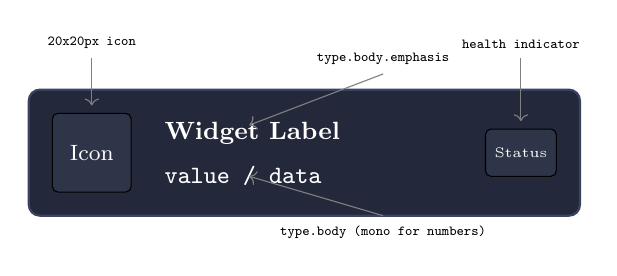
\begin{tikzpicture}[
  every node/.style={font=\small},
]
% Widget container
\draw[rounded corners=4pt, fill=surface, draw=outline, thick]
  (0, 0) rectangle (7, 1.6);

% Icon area
\draw[fill=surfaceraised, rounded corners=2pt]
  (0.3, 0.3) rectangle (1.3, 1.3);
\node[font=\footnotesize, color=white] at (0.8, 0.8) {Icon};

% Label
\node[anchor=west, font=\small\bfseries, color=white] at (1.6, 1.05) {Widget Label};

% Value
\node[anchor=west, font=\small\ttfamily, color=white!70] at (1.6, 0.5) {value / data};

% Health indicator area
\draw[fill=surfaceraised, rounded corners=2pt]
  (5.8, 0.5) rectangle (6.7, 1.1);
\node[font=\tiny, color=white] at (6.25, 0.8) {Status};

% Annotations
\draw[<-, gray, thin] (0.8, 1.4) -- (0.8, 2.0) node[above, font=\tiny\ttfamily, black] {20x20px icon};
\draw[<-, gray, thin] (2.8, 1.15) -- (4.5, 1.8) node[above, font=\tiny\ttfamily, black] {type.body.emphasis};
\draw[<-, gray, thin] (2.8, 0.5) -- (4.5, 0.0) node[below, font=\tiny\ttfamily, black] {type.body (mono for numbers)};
\draw[<-, gray, thin] (6.25, 1.2) -- (6.25, 2.0) node[above, font=\tiny\ttfamily, black] {health indicator};

\end{tikzpicture}
\caption{Widget base structure in Visible prominence. Actual content varies per widget type.}
\label{fig:widget-anatomy}
\end{figure}

\subsection{Health State Visual Treatment}

Every widget wraps its content in the shared degraded-state QML component, which applies visual treatments based on the \texttt{status} field from the daemon. The degraded-state system uses three complementary channels to communicate widget health without sacrificing readability:

\begin{enumerate}[leftmargin=1.5em, itemsep=3pt]
  \item \textbf{Left-edge status pill.} A 2px-wide vertical bar on the left edge of the widget container, constrained to the vertical height of the widget's title area (not the full widget height). The pill uses muted, desaturated versions of the semantic state colors---not the full-saturation \texttt{warning}/\texttt{error} tokens. This provides at-a-glance scannability: a user can sweep their eyes across the bar and immediately identify which widgets have issues by the presence and color of the pill.

  \item \textbf{Content desaturation (no opacity change).} Text opacity and background color remain identical to the \texttt{Normal} state---readability is never compromised. Instead, all chromatic content within the widget (colored icons, chart fills, tag badges, sparkline colors) is rendered in grayscale or monochrome (\texttt{fg.muted}). This creates a ``powered down'' look that is visually distinct without reducing legibility.

  \item \textbf{Status indicator icon.} A small icon in the top-right corner of the widget provides concrete confirmation of the state, which is essential for colorblind users who may not distinguish the pill colors. The icon is the definitive, accessible signal.
\end{enumerate}

\begin{longtable}{p{2.2cm} p{2.5cm} p{2cm} p{6.5cm}}
\toprule
\textbf{State} & \textbf{Left Pill} & \textbf{Icon} & \textbf{Details} \\
\midrule
\texttt{Normal} & None & None & Default appearance. Full color saturation, no indicators. \\
\addlinespace
\texttt{Stale} & 2px pill, muted slate (\texttt{fg.subtle}) & Clock (10px, \texttt{fg.muted}) & All chromatic content desaturated to grayscale. Tooltip reads ``Data from [timestamp] --- last update [duration] ago.'' Data is still displayed (last known good). On transition to Stale, the clock icon pulses once via \texttt{spring.snappy} to draw attention, then rests. \\
\addlinespace
\texttt{Error} & 2px pill, muted terracotta (desaturated \texttt{warning}) & Warning triangle (10px, \texttt{warning}) & All chromatic content desaturated to grayscale. Tooltip shows the error message. Clicking the warning icon offers retry or opens module settings. No pulse on the icon---errors are persistent states, not events. \\
\addlinespace
\texttt{Unavailable} & None & None & Widget is hidden entirely. No placeholder, no error state---it simply doesn't exist in the layout. \\
\bottomrule
\end{longtable}

\begin{designbox}[Pill Color Tokens]
The left-edge pill uses dedicated muted color tokens, not the raw state colors:
\begin{itemize}[leftmargin=1.5em, itemsep=2pt]
  \item \texttt{state.stale.pill}: A desaturated cool gray derived from \texttt{fg.subtle}. Should be visible against \texttt{surface} but not attention-grabbing.
  \item \texttt{state.error.pill}: A desaturated warm tone (muted terracotta) derived from \texttt{warning} at $\sim$40\% saturation. Warmer than the stale pill, distinguishable at a glance, but not alarming.
\end{itemize}
These are separate tokens so theme authors can tune them independently. The full-saturation \texttt{warning} and \texttt{error} tokens are reserved for the urgency/escalation system (Section~\ref{sec:urgency}), where they signal actionable conditions. Health state pills signal data freshness, which is a lower-urgency concern.
\end{designbox}

\subsubsection{Desaturation Implementation Strategy}

The content desaturation described above can be implemented at two quality levels:

\begin{enumerate}[leftmargin=1.5em, itemsep=3pt]
  \item \textbf{Full shader (quality mode).} A QML layer effect (\texttt{DesaturateEffect}) renders the widget to an offscreen framebuffer and applies a grayscale shader. This desaturates \emph{all} chromatic content---icons, sparkline charts, colored tags, progress bars---uniformly. However, each active layer effect consumes GPU resources (one offscreen render pass per affected widget). If multiple widgets enter degraded states simultaneously (e.g., a network drop affects several network-dependent widgets), the cumulative cost may cause frame drops on integrated GPUs.

  \item \textbf{Token swap (performance mode).} Instead of a real-time shader, the wrapper overrides color tokens within the widget's scope: icon color is set to \texttt{fg.muted}, text color remains at \texttt{fg}, and any widget-internal accent colors (sparkline fill, tag background) are overridden to \texttt{fg.muted} or \texttt{outline}. This achieves the ``powered down'' look with zero GPU overhead but cannot desaturate arbitrary rendered content (e.g., a raster thumbnail or a complex SVG chart would retain its original colors).
\end{enumerate}

The implementation should use \textbf{token swap by default} and offer the full shader as an opt-in via a theme token (\texttt{health.desaturation\_mode = "shader"} or \texttt{"token\_swap"}). On battery, the system always falls back to token swap regardless of the setting. The visual difference between the two modes is negligible for typical bar widgets (which are composed of icons and text), and only becomes apparent for widgets with complex colored content like embedded charts.


% ===========================================================================
\section{Iconography}
\label{sec:icons}

\subsection{Icon Set}

Levshell uses \textbf{Phosphor Icons} in the \textbf{regular (outlined) weight} as its icon set. Phosphor provides over 6,000 icons with clean outlined strokes, comprehensive coverage of academic and developer-relevant glyphs (flask, books, terminal, git-branch, brain, graduation-cap, chart-line, etc.), and availability as both a web font and individual SVGs.

The regular (outlined) weight is the default. Its thin, consistent strokes complement Spectral's serif character without competing for visual weight. The outlined style also reads well at the small sizes used in the bar (16--20px).

\begin{designbox}[Duotone as Theme Option]
Phosphor offers a \textbf{duotone} variant where secondary icon elements render at reduced opacity, creating a two-tone effect. This is available as an opt-in theme option (\texttt{icon\_style = "duotone"} in the theme TOML) but is \emph{never} the default. The default is single-color outlined icons. Theme authors who enable duotone must ensure the secondary tone uses \texttt{fg.muted} or an equivalently subtle color---duotone icons should add depth, not introduce visual noise.
\end{designbox}

\subsection{Icon Sizes}

\begin{longtable}{p{3cm} p{2cm} p{8.5cm}}
\toprule
\textbf{Context} & \textbf{Size} & \textbf{Notes} \\
\midrule
Bar widget (full) & 20px & Inside widget containers. Consistent across all widgets. \\
Bar widget (compact) & 16px & Reduced with density \\
Dropdown list item & 20px & List rows in panels \\
Command palette result & 24px & Larger for scannability \\
Quick-settings tile & 24px & Toggle icons \\
Notification icon & 28px & App icon in notification entries \\
Tooltip / status & 10px & Degraded-state indicators (clock, warning triangle) \\
Badge dot & 6px & \texttt{Badge} prominence level (colored circle, no icon) \\
\bottomrule
\end{longtable}

Icon sizes are consistent within each context---all bar widgets use 20px in full density, not variable sizes based on importance. Visual hierarchy is communicated through prominence levels and the urgency/escalation system, not through icon size variation.

\subsection{Icon Color Behavior}

Icons inherit their color from the text color of their context:
\begin{itemize}[leftmargin=1.5em, itemsep=2pt]
  \item Default: \texttt{fg} (primary foreground)
  \item Inactive/disabled: \texttt{fg.muted}
  \item Ambient escalation (Section~\ref{sec:urgency}): \texttt{fg.muted} (dimmer than default)
  \item On primary background: \texttt{on.primary}
  \item State-specific: \texttt{success}, \texttt{warning}, \texttt{error} as appropriate (e.g., the battery icon turns \texttt{warning} below 20\%, \texttt{error} below 5\%)
\end{itemize}

In the default outlined style, icons are \textbf{single-color}, matching their context. When the duotone theme option is enabled, the primary stroke uses the context color and the secondary fill uses \texttt{fg.muted} (or a theme-specified duotone secondary color). Even in duotone mode, state-specific coloring overrides both tones---a battery icon at \texttt{error} level renders entirely in \texttt{error} color, not in duotone.


% ===========================================================================
\section{Urgency and Escalation Grammar}
\label{sec:urgency}

This is the visual vocabulary for the ``quiet until important'' principle. It defines how widgets transition from ambient background presence to active attention demand.

\subsection{Escalation Levels}

\begin{longtable}{p{2.5cm} p{3.5cm} p{7.5cm}}
\toprule
\textbf{Level} & \textbf{Visual Treatment} & \textbf{Examples} \\
\midrule
\texttt{Ambient} & Monochrome icon/text in \texttt{fg.muted}. May be in \texttt{IconOnly} or \texttt{Compact} prominence. & CPU at 20\%, battery at 80\%, no SSH connections. Normal resting state. \\
\addlinespace
\texttt{Aware} & Icon/text in \texttt{fg} (full foreground). Prominence may increase to \texttt{Visible}. & CPU crosses 60\%, battery drops below 30\%, meeting in 15 minutes. \\
\addlinespace
\texttt{Attention} & Icon/value gains \texttt{warning} color. A subtle badge or dot may appear. Prominence may increase to \texttt{Expanded}. & CPU at 90\%, battery at 10\%, SSH connection dropped, Anki cards overdue by 2 days. \\
\addlinespace
\texttt{Critical} & Icon/value gains \texttt{error} color. The widget's left-edge pill flashes once in full-saturation \texttt{error} color (a single brief flash via \texttt{spring.snappy}, settling to static \texttt{error} color). A notification is also emitted. & Battery at 3\%, disk space critically low, SSH tunnel died during active use. \\
\bottomrule
\end{longtable}

\subsection{Rules}

\begin{enumerate}[leftmargin=1.5em, itemsep=3pt]
  \item Escalation is always gradual: \texttt{Ambient} $\to$ \texttt{Aware} $\to$ \texttt{Attention} $\to$ \texttt{Critical}. No widget jumps from \texttt{Ambient} to \texttt{Critical}.
  \item De-escalation is faster than escalation (the context engine's hysteresis deactivation delay handles this).
  \item A widget at \texttt{Critical} emits a notification. The notification is the user's escape hatch if they've hidden the widget or aren't looking at the bar.
  \item During a focus session (Do Not Disturb active), \texttt{Attention} and \texttt{Critical} levels are still applied visually in the bar, but notifications are silenced and queued.
  \item The border flash at \texttt{Critical} fires once when the level is entered. It never repeats. After the flash settles, the left-edge pill remains at static \texttt{error} color. No looping, no flashing, no pulsing.
  \item The escalation system's left-edge pill uses \emph{full-saturation} state colors (\texttt{warning}, \texttt{error}), unlike the health state system's muted pills (Section~\ref{sec:widgets}). Escalation demands attention; health state communicates data freshness. The visual intensity difference between these two pill systems is deliberate.
\end{enumerate}


% ===========================================================================
\section{Focus and Ambient Mode}
\label{sec:focus}

\subsection{Focus Session Visual Shift}

When a focus session is active (Pomodoro running, or Do Not Disturb manually engaged), the bar's visual tone shifts through two complementary channels:

\begin{enumerate}[leftmargin=1.5em, itemsep=3pt]
  \item \textbf{Content muting (primary signal).} All non-critical widget content shifts to \texttt{fg.muted}. Icons, labels, and values for widgets below \texttt{Attention} escalation level are rendered in the muted foreground color. Only widgets at \texttt{Attention} or \texttt{Critical} retain full-color rendering. This is the dominant visual cue that focus mode is active---the bar feels ``dimmed down'' without any loss of readability for the information that matters.

  \item \textbf{Subtle opacity decrease (secondary signal, blur mode only).} In blur mode, bar opacity decreases by 5\% (e.g., from 80\% to 75\%), making the bar very slightly more transparent. This is a background-level cue, not the primary indicator---most users will perceive the content muting first. In opaque mode (battery or blur disabled), the bar background shifts from \texttt{surface} to \texttt{bg} (one tier darker in the surface hierarchy), producing an equivalent ``recessed'' effect without relying on transparency.
\end{enumerate}

\textbf{Notification badge} shows a ``paused'' indicator (a small Phosphor pause icon replacing the unread count) to signal that notifications are being queued, not lost.

The transition into focus mode uses \texttt{spring.default} ($\sim$200ms settle) for spatial changes and critically damped fades for color shifts.

\subsubsection{Visual State Stacking Rule}

Focus mode content muting, health state desaturation, and escalation coloring are three independent visual systems that can apply to the same widget simultaneously. To prevent a widget from becoming invisible when multiple systems stack, the following precedence rule applies:

\begin{enumerate}[leftmargin=1.5em, itemsep=3pt]
  \item \textbf{Escalation color takes absolute precedence.} If a widget is at \texttt{Attention} or \texttt{Critical} escalation, it renders in full escalation color (\texttt{warning} or \texttt{error}) regardless of focus mode or health state. The user needs to see critical information.

  \item \textbf{Health state treatment overrides focus muting.} If a widget is in \texttt{Stale} or \texttt{Error} health state, its health state appearance (left-edge pill, desaturation, status icon) is rendered as specified in Section~\ref{sec:widgets}---focus mode does \emph{not} further mute its content. The health state visual treatment already communicates ``this widget is degraded''; additional focus-mode dimming would reduce it to near-invisibility and destroy the legibility guarantee.

  \item \textbf{Focus muting applies to healthy, non-escalated widgets only.} The \texttt{fg.muted} color shift applies only to widgets that are simultaneously in \texttt{Normal} health state \emph{and} below \texttt{Attention} escalation level. This is the common case (most widgets, most of the time) and produces the intended ``dimmed down'' bar.
\end{enumerate}

In short: escalation $>$ health state $>$ focus muting. A widget is never affected by more than one of these systems at a time.

A persistent visual cue in the bar communicates that a focus session is active. The user selects their preferred indicator style via configuration (\texttt{focus.indicator\_style} in \texttt{levshell.toml}). The default is \texttt{bottom-edge-line}.

\begin{longtable}{p{3.5cm} p{10cm}}
\toprule
\textbf{Style} & \textbf{Description} \\
\midrule
\texttt{bottom-edge-line} (default) & A thin line (2px, \texttt{primary}) along the bottom edge of the bar, facing the desktop content. Subtle, always visible at a glance, and clearly signals ``the bar is in a special mode'' without consuming any bar space. \\
\addlinespace
\texttt{top-edge-line} & A thin line (2px, \texttt{primary}) along the top edge of the bar. More hidden (against the screen edge), but some users may prefer the indicator to be out of their primary visual field. \\
\addlinespace
\texttt{pill} & A small pill-shaped badge next to the clock reading ``Focusing'' or showing elapsed focus time. More explicit and informational but consumes bar space. Text uses \texttt{type.label} in \texttt{primary} color on a \texttt{surface.raised} background. \\
\addlinespace
\texttt{clock-replace} & The clock switches from displaying wall time to elapsed focus time (e.g., ``1:23:07''). Wall time moves to the clock's tooltip. Zero additional bar space consumed. The most space-efficient option but obscures the current time. \\
\bottomrule
\end{longtable}

\subsection{Presentation / Screen-Sharing Mode}

A special mode that strips the bar to absolute essentials:

\begin{itemize}[leftmargin=1.5em, itemsep=3pt]
  \item Only clock and recording indicator are visible.
  \item Notification content is hidden (badges show counts but not text).
  \item Calendar, inbox, and project details are suppressed to avoid leaking personal information.
  \item The bar may optionally switch to compact density automatically.
\end{itemize}

\subsection{Break Period}

During a Pomodoro break, the bar returns to normal visual treatment (content muting lifts, opacity returns to default), and a break indicator replaces the focus indicator:

\begin{itemize}[leftmargin=1.5em, itemsep=2pt]
  \item A configurable break icon (\texttt{focus.break\_icon} in \texttt{levshell.toml}) appears in the bar in \texttt{success} color. Options: \texttt{coffee} (default), \texttt{leaf}, \texttt{pause}, or any valid Phosphor icon name. The default is \texttt{coffee} because coffee is non-negotiable.
  \item Screen may dim to a configurable level (e.g., 70\% brightness) as a gentle physical reminder to rest eyes.
\end{itemize}


% ===========================================================================
\section{Theming Architecture}
\label{sec:theming}

\subsection{Theme File Structure}

Themes are TOML files under \texttt{\textasciitilde/.config/levshell/themes/}. Each file defines a single variant (dark or light) and supplies concrete values for all tokens. A complete theme \emph{package} may consist of two files (e.g., \texttt{warm-dark.toml} and \texttt{warm-light.toml}), but each file is self-contained and independently valid. Dark mode is the primary design target; light mode themes are supported but secondary.

Levshell ships with three built-in themes: \texttt{warm-dark.toml} (default), \texttt{neutral-dark.toml}, and \texttt{warm-light.toml}.

\begin{lstlisting}[language={}]
# ~/.config/levshell/themes/warm-dark.toml (default theme)

[meta]
name = "Warm Dark"
author = "Levshell"
variant = "dark"              # "dark" or "light"
light_pair = "warm-light"     # optional: paired light theme name

# --- Surface Hierarchy (4-tier) ---
[colors]
bg = "#1A1B26"
bg.dark = "#16161E"
surface = "#24283B"
surface.raised = "#2F3549"
overlay = "#3B4261"

# --- Content Colors ---
fg = "#C0CAF5"
fg.muted = "#565F89"
fg.subtle = "#737AA2"
on.primary = "#1A1B26"
on.surface = "#C0CAF5"
outline = "#3B4261"

# --- Accent Colors (single primary) ---
primary = "#7AA2F7"
primary.variant = "#5A7FD4"
secondary = "#BB9AF7"
secondary.variant = "#9D7CD8"
tertiary = "#7DCFFF"

# --- State Colors ---
success = "#9ECE6A"
warning = "#E0AF68"
error = "#F7768E"
info = "#2AC3DE"

# --- Health State Pills (muted, desaturated) ---
[health]
stale.pill = "#737AA2"        # derived from fg.subtle
error.pill = "#B8806A"        # muted terracotta, ~40% sat warning

# --- Bar Geometry & Blur ---
[bar]
opacity = 0.80
blur_radius = 30              # px, 0 = opaque
opacity_battery = 1.0
blur_radius_battery = 0
height_full = 44
height_compact = 32

# --- Typography ---
[typography]
font_text = "Spectral"
font_mono = "IBM Plex Mono"

# --- Icons ---
[icons]
style = "outlined"            # "outlined" or "duotone"
duotone_secondary = "#565F89" # only used when style = "duotone"

# --- Motion ---
[motion]
reduce_motion = false
\end{lstlisting}

\subsubsection{Required vs.\ Optional Sections}

A valid theme file \textbf{must} define \texttt{[meta]} and \texttt{[colors]}. All other sections are optional and fall back to the built-in default values if omitted. This means a minimal community theme can supply just a color palette and inherit all other tokens from the defaults.

\subsubsection{Focus and Break Configuration}

Focus indicator style and break icon are \emph{user preferences}, not theme properties. They live in the global \texttt{levshell.toml}, not in theme files:

\begin{lstlisting}[language={}]
# ~/.config/levshell/levshell.toml (excerpt)

[focus]
indicator_style = "bottom-edge-line"  # see Section 10.1
break_icon = "coffee"                 # any valid Phosphor icon name
break_dim_brightness = 0.70           # screen dim during breaks
\end{lstlisting}

This separation ensures that switching themes does not reset the user's focus preferences, and that focus behavior is consistent regardless of which theme is active.

\subsection{Dark and Light Mode}

Dark mode is the default and primary mode. Light mode is supported for users who prefer it or who work in bright environments, but all design decisions in this document are validated against the dark palette first.

Each mode is a separate theme file. The \texttt{light\_pair} field in \texttt{[meta]} optionally names the corresponding light variant, enabling a single keybind or \texttt{levshell-ctl theme toggle-mode} to switch between them. If no pair is specified, toggling mode has no effect.

Light mode themes invert the luminance relationships: backgrounds become light, surfaces become off-white, and foreground text becomes dark. Accent colors remain the same hue but may shift in lightness or saturation to maintain contrast. The light palette is hand-authored, not algorithmically derived---automatic inversion produces poor results for warm palettes.

A \texttt{Theme.mode} token (\texttt{"dark"} or \texttt{"light"}) is exposed to QML and derived from the active theme's \texttt{variant} field. Toggling is instant (no cross-fade) and propagated to the global color scheme sync system when that feature is available (Phase~2+).

\subsection{Global Color Scheme Propagation}

When a theme is activated, the daemon propagates the color scheme to:

\begin{enumerate}[leftmargin=1.5em, itemsep=2pt]
  \item \textbf{Sway borders:} Updates \texttt{client.focused}, \texttt{client.unfocused}, etc.\ in the Sway config or via Sway IPC.
  \item \textbf{GTK:} Writes \texttt{settings.ini} or uses \texttt{gsettings} to set the preferred color scheme.
  \item \textbf{Qt:} Sets environment variables or writes \texttt{qt5ct}/\texttt{qt6ct} configuration.
  \item \textbf{Terminals:} Optionally writes a colorscheme file for the configured terminal emulator (Alacritty, Kitty, foot).
\end{enumerate}

This is a Phase~2+ feature. In Phase~1, the theme file is read by the QML shell directly and only applied to Levshell's own surfaces.


% ===========================================================================
\section{Dropdown and Overlay Surfaces}
\label{sec:overlays}

\subsection{Shared Anatomy}

All dropdown panels, flyouts, and overlays share structural properties:

\begin{itemize}[leftmargin=1.5em, itemsep=2pt]
  \item Background: \texttt{surface} at \texttt{bar.opacity} with backdrop blur (blur mode), or opaque \texttt{surface} (opaque/battery mode).
  \item Corner radius: 8px.
  \item Shadow: \texttt{0 4px 16px rgba(0,0,0,0.3)}.
  \item Border: 1px \texttt{outline}.
  \item Internal padding: \texttt{space.lg} (12px).
  \item Animation: open with \texttt{spring.default}, close with \texttt{spring.snappy}. Opacity fades use linear interpolation at \texttt{motion.fast}.
  \item Dismissal: click outside, Escape key, or re-click the triggering widget.
\end{itemize}

\subsection{Command Palette}

The command palette is a special overlay---centered on screen (not anchored to a bar widget), wider (550--650px), and taller (up to 50\% screen height). It has a prominent search input at the top with large type (\texttt{type.title}), and results below in categorized sections with \texttt{type.body} text and 24px icons. The selected result has a \texttt{surface.raised} background. The command palette uses the same 8px corner radius and blur/opacity treatment as other overlays---it is visually distinguished by its size and centered positioning, not by special styling.

\subsection{Notification Center}

Anchored to the notification icon in the bar. Width: 380px. Notifications are grouped by application with collapsible headers. Each notification entry has: app icon (28px), title (\texttt{type.body.emphasis}), body (\texttt{type.body}), timestamp (\texttt{type.caption}, \texttt{fg.muted}), and action buttons. Unread notifications have a small \texttt{primary} dot. The Do Not Disturb toggle is at the top of the panel.

\subsection{Quick-Settings Flyout}

Anchored to a system tray icon. Width: 340px. Organized as a grid of toggle tiles (2 columns). Each tile has a 24px icon, a label (\texttt{type.label}), and a toggle state (on = \texttt{primary} background, off = \texttt{surface.raised}). Sliders (volume, brightness) span the full width with a track in \texttt{outline} and a fill in \texttt{primary}.


% ===========================================================================
\section{Implementation Notes}
\label{sec:implementation}

\subsection{Token Delivery to QML}

All design tokens are exposed as properties on a global \texttt{Theme} QML singleton:

\begin{lstlisting}[language={}]
// In QML
Text {
    text: "CPU 72%"
    color: Theme.fg
    font.family: Theme.fontMono
    font.pixelSize: Theme.typeBody
}

Rectangle {
    color: Theme.surface
    opacity: Theme.barOpacity
    radius: 8
}
\end{lstlisting}

The \texttt{Theme} singleton reads from the active theme TOML file (via the daemon or directly) and exposes every token as a QML property. Changing themes updates all properties, and QML's binding system propagates the changes to every referencing component automatically.

\subsection{Degraded-State Wrapper Component}

A reusable QML component that wraps any widget and applies the health state visual treatment:

\begin{lstlisting}[language={}]
// WidgetWrapper.qml (pseudocode)
Item {
    property string status: "normal"  // from daemon
    property alias content: contentLoader.sourceComponent

    // No opacity change -- readability is never compromised
    opacity: 1.0

    // Left-edge status pill (partial height, aligned to title area)
    Rectangle {
        visible: status !== "normal"
        width: 2
        height: parent.titleAreaHeight  // pill, not full border
        color: status === "stale" ? Theme.staleStatePill
             : status === "error" ? Theme.errorStatePill
             : "transparent"
    }

    // Desaturation: token swap (default) or shader (opt-in)
    // Token swap: override color tokens for child content
    property color iconColor: status !== "normal" ? Theme.fgMuted
                            : Theme.fg
    property color accentColor: status !== "normal" ? Theme.outline
                              : Theme.primary

    // Shader mode (opt-in via health.desaturation_mode = "shader")
    // Uncomment to enable full GPU-based desaturation:
    // layer.enabled: status !== "normal"
    // layer.effect: DesaturateEffect {
    //     desaturation: status !== "normal" ? 1.0 : 0.0
    // }

    // Status indicator icon (top-right corner)
    StatusIcon {
        visible: status !== "normal"
        icon: status === "stale" ? "clock"
            : status === "error" ? "warning-triangle"
            : ""
        size: 10
        color: status === "stale" ? Theme.fgMuted
             : status === "error" ? Theme.warning
             : "transparent"
    }

    Loader { id: contentLoader }
}
\end{lstlisting}

Every widget in \texttt{shell/widgets/} uses this wrapper. The wrapper is implemented once, tested once, and guarantees visual consistency across all health states. In the default token-swap mode, the wrapper overrides color properties that child components bind to (icon color, accent color); individual widgets do not need to implement health-state logic. In shader mode, the QML layer effect desaturates all rendered content, including complex visuals like charts.


\end{document}
